\documentclass[12pt]{article}
\usepackage[T1]{fontenc}
\usepackage{graphicx}
\usepackage{amsmath}
\usepackage{fancyhdr}
\usepackage{geometry}
\geometry{
  top=0.7in,            % <-- you want to adjust this
  inner=0.5in,
  outer=0.5in,
  bottom=0.5in,
  headheight=3ex,       % <-- and this
  headsep=2ex,          % <-- and this
}
\pagestyle{fancy}
\lhead{Digital Image processing}
\chead{HW2}

\rhead{Aryan Mikaeili (95105895)}
\newlength{\drop}

\begin{document}
  \begin{titlepage}
\drop=0.1\textheight
    \centering
	
    \vspace*{\baselineskip}
	\begin{center}
	  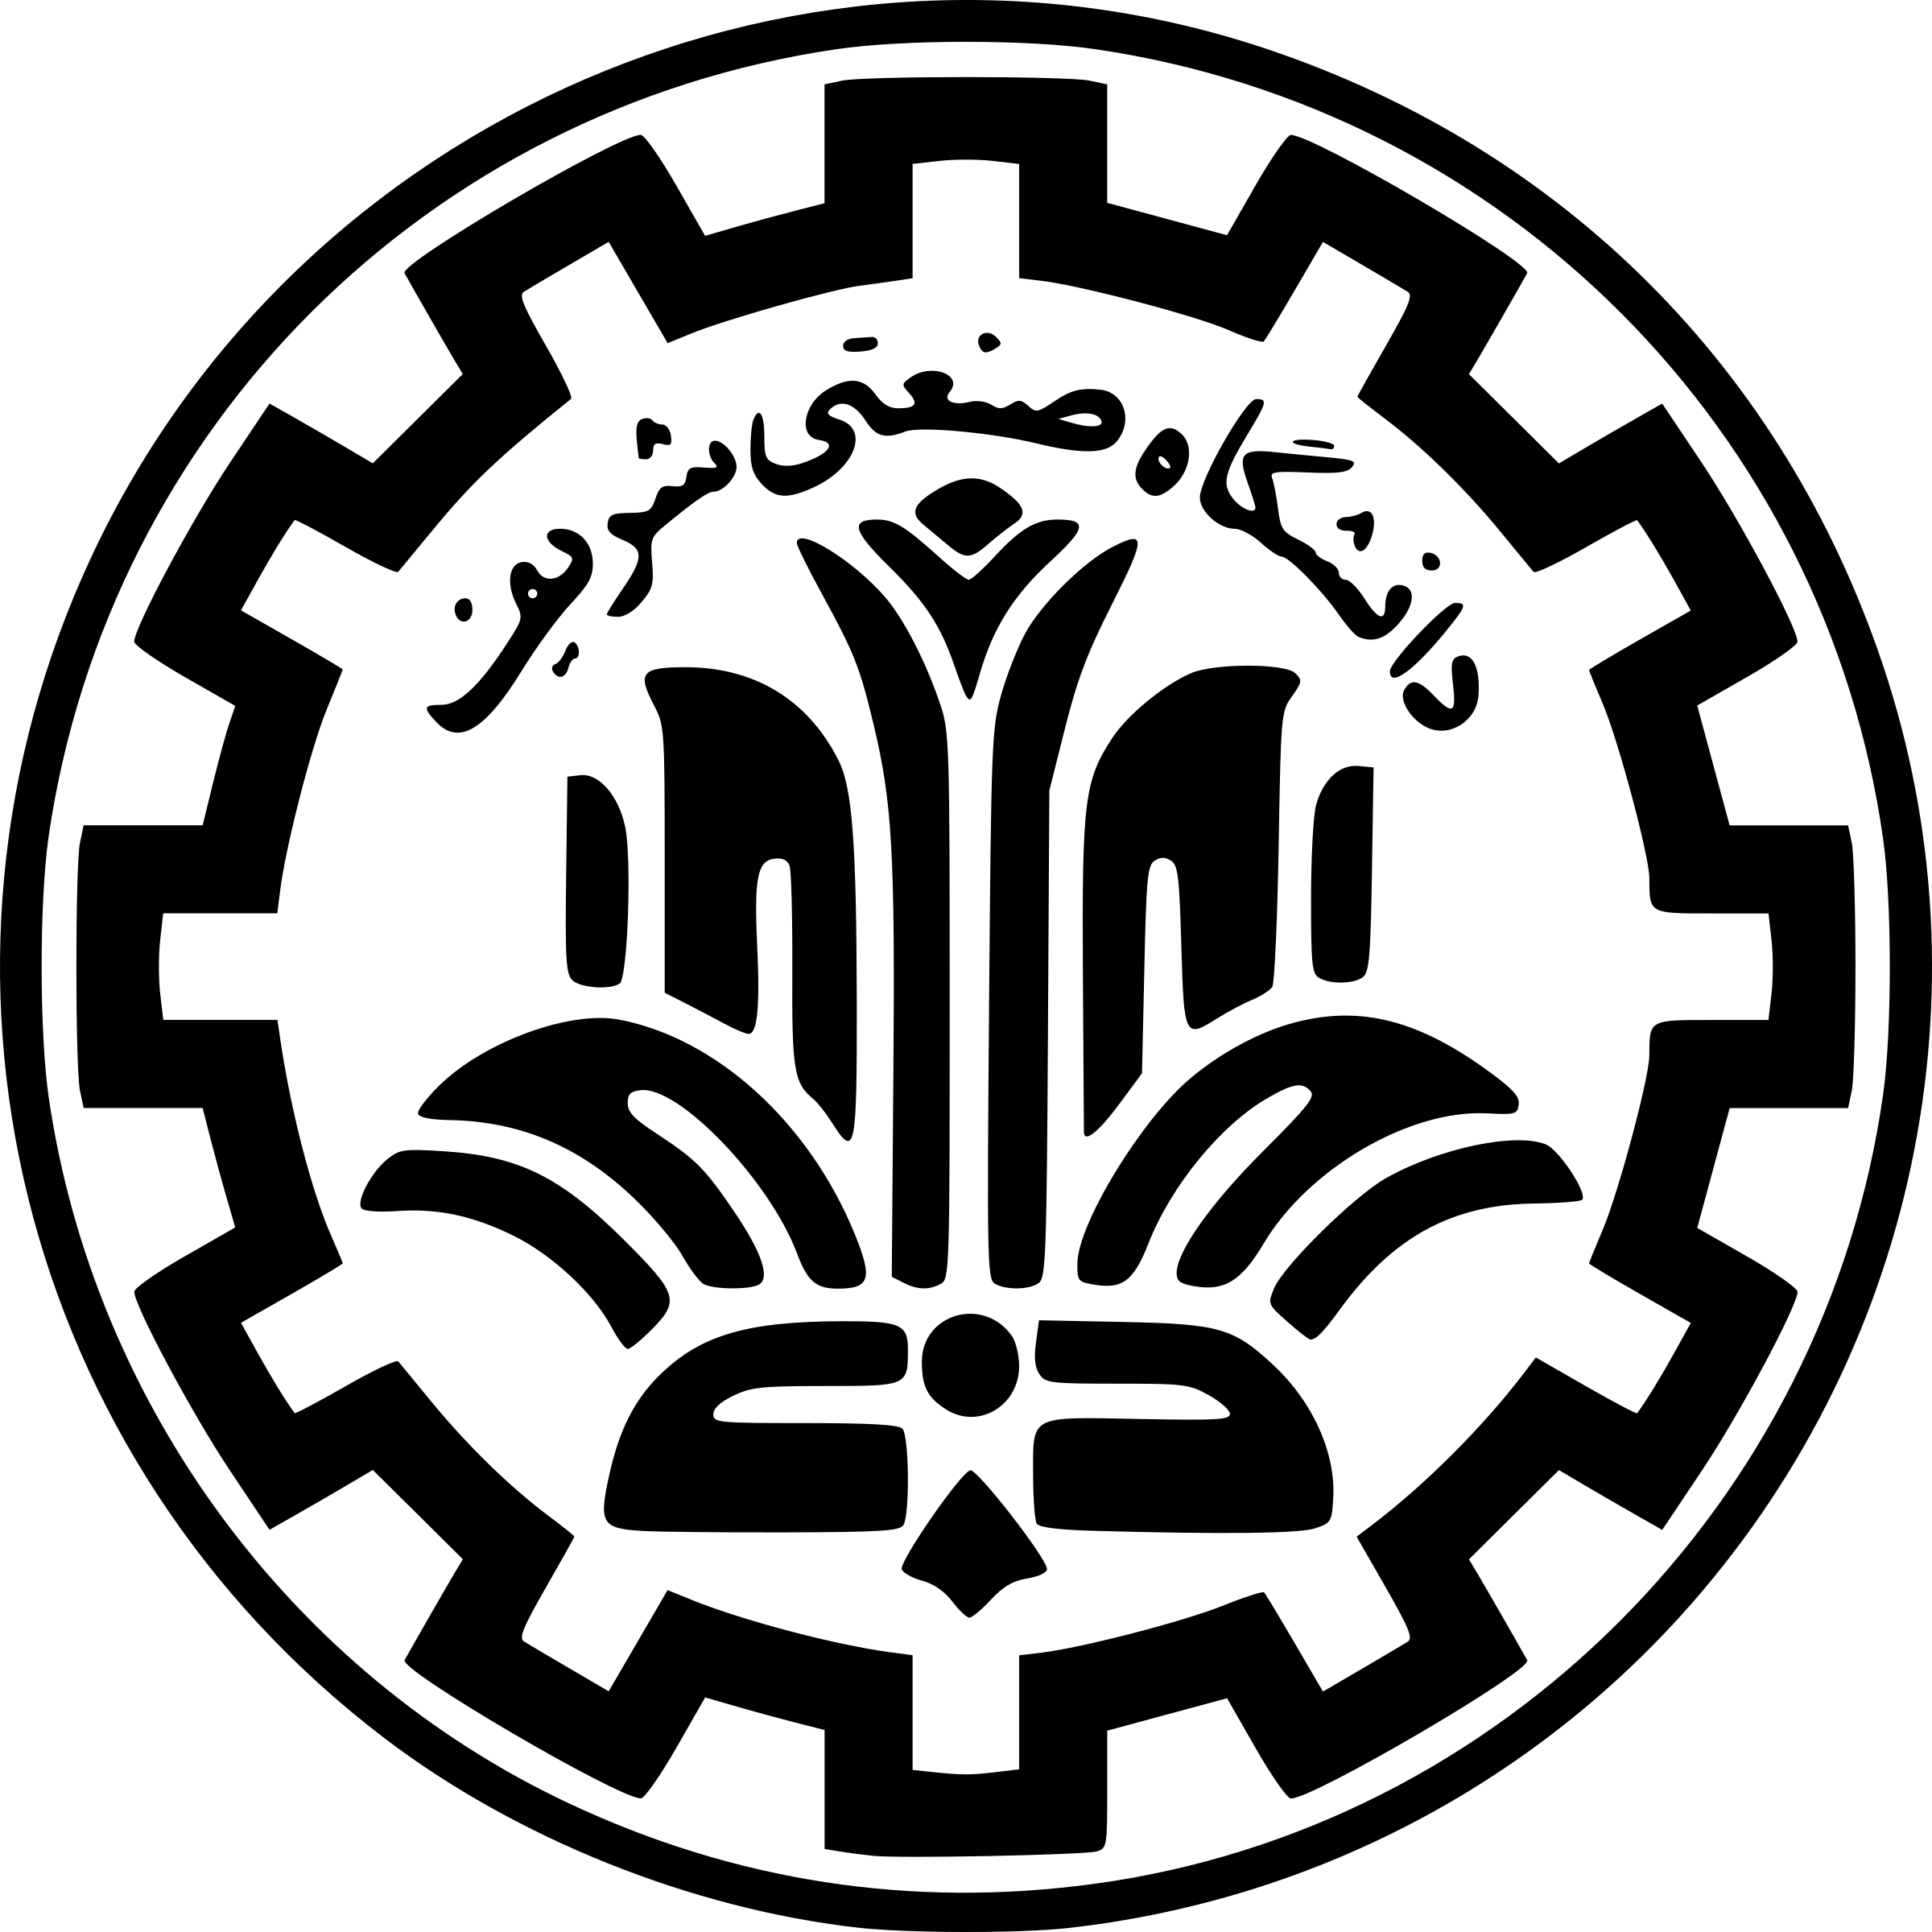
\includegraphics[width=200pt]{logo.png}
	\end{center}
    \rule{\textwidth}{1.6pt}\vspace*{-\baselineskip}\vspace*{2pt}
    \rule{\textwidth}{0.4pt}\\[\baselineskip]
    {\LARGE Digital Image Processing }\\[0.2\baselineskip]
    \rule{\textwidth}{0.4pt}\vspace*{-\baselineskip}\vspace{3.2pt}
    \rule{\textwidth}{1.6pt}\\[\baselineskip]
\vspace*{2\baselineskip}
    \scshape
	{\LARGE Homework 2}


    \par
\vspace*{2\baselineskip}
    \scshape
	Professor: Dr. Shohreh Kasaei
    \par

    \vspace*{2\baselineskip}

   {\Large Aryan Mikaeili (95105895)\par}
\vspace*{2\baselineskip}
\today
   	

 
  \end{titlepage}

\vspace*{-\baselineskip}
\section{}
 The maximum frequency present in the signal as shown in the right hand side plot is approximately equal to \textbf{5800 Hz}.
According to Nyquist theory the sampling rate must at least be twice the maximum frequency size of the signal for us to be able to reconstruct the signal form the sampled output. this theory will be discussed thoroughly in question 2. therefore:
$$ F_s > 2 \times F_c$$
$$F_c  = 5800 Hz \Rightarrow F_s > 11600 Hz \Rightarrow min(F_s) = 11600$$
Here, $F_c$ is the cutoff frequency of the signal in frequency domain.

\section{}
First of all, we shall discuss the Nyquist theory, and then the definition of aliasing will come naturally.

Suppose we have a continuous signal $x(t)$ which is bandlimited, i.e. it has value in some range and it is zero otherwise.
for sampling this signal, we must multiply this function to a impulse train. let's call this function $p$.
$$p =  \sum_{n = -\infty}^{n = \infty} \delta(t - nT) $$
$$ x_s(n) = x(nT) = x(t) \times \sum_{n = -\infty}^{n = \infty} \delta(t - nT) $$

these signals, have fourier transforms as written below:
$$ X(j\omega) = \int_{t = -\infty}^{t = \infty} x(t) \exp(j\omega t) dt$$
$$P(jw) = \frac{2\pi}{T}\sum_{n = -\infty}^{n = \infty} \delta(w - w_s n)$$
where $\omega_s = \frac{2\pi}{T}$ and $T$ is the sampling period.
we also know that multiplication in the time domain, is equivalent to convolution in frequency domain. so we have:
$$X_s(j\omega) = \frac{1}{2\pi} (X(j\omega) * P(jw))$$

For example, suppose our signal is what we have depicted in the figure below. Also, the impulse train is depicted. the convolution of the two functions will result in copied versions of the function $X(j\omega)$, with period $\omega_s$. this function, is the sampled function in frequency domain. Hence for the reconstruction of the continuous signal, we just have to multiply $X_{s}(j\omega)$ by a lowpass filter with gain $T$ and a cutoff frequency, greater than $\omega_c$ and less than $\omega_s - \omega_c$.



	\begin{center}
	  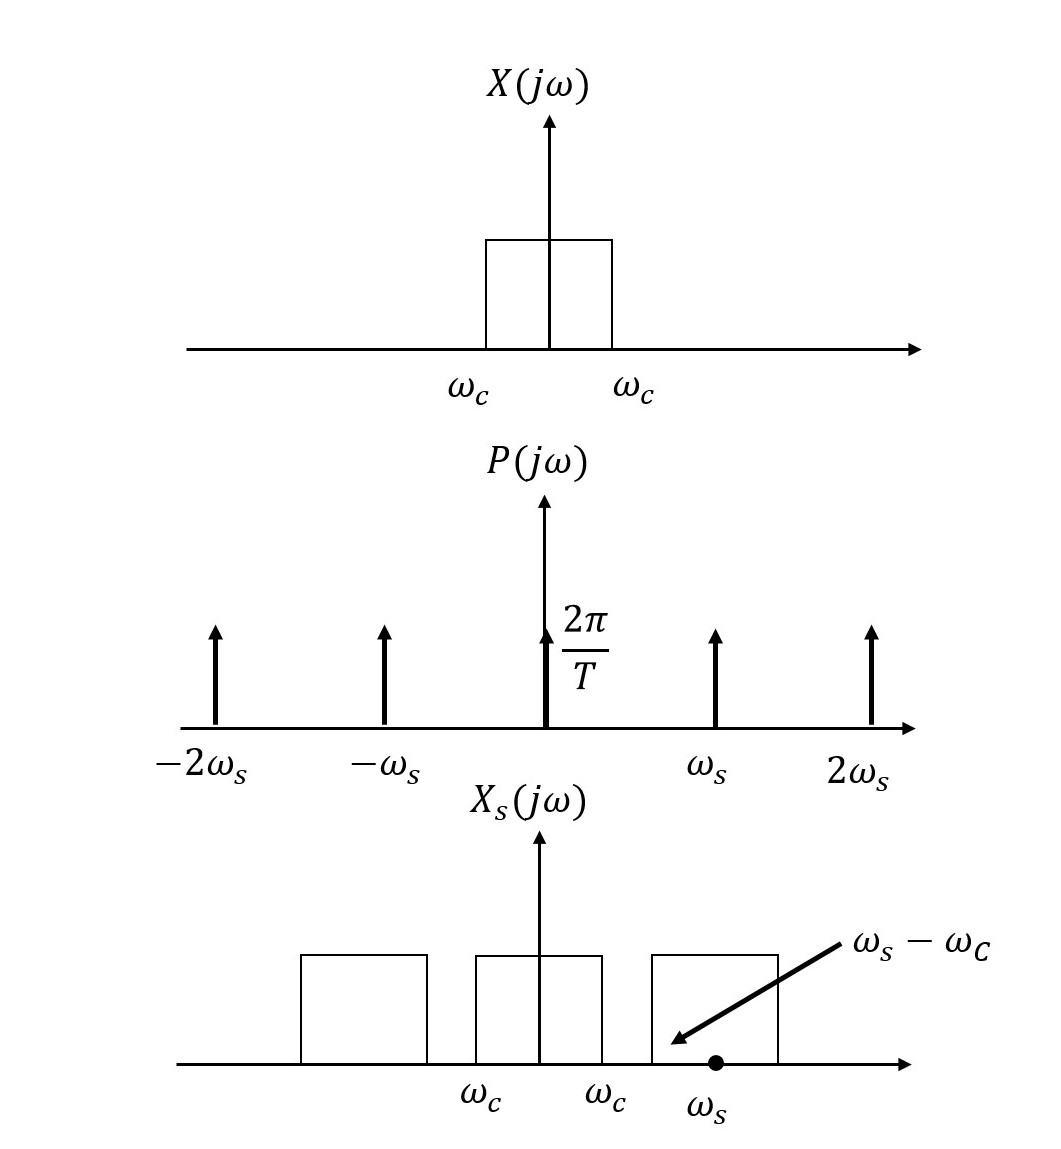
\includegraphics[width=200pt]{fig1.jpg}
	\label{fig_1}
	\end{center}

But all of these is valid if the space between the two copied versions in the $X_{s}(j\omega)$ plot is greater than zero. That is:
$$ (\omega_s - \omega_c) - \omega_c \geq 0 \Rightarrow \omega_s \geq 2 \omega_c$$.
If this is not the case, by multiplying the sampled function, with a lowpass filter, we would not be able to reconstruct the continuous signal and depending on how lower our sampling fequency is from the cutoff frequency of the signal, by filtering the sampled function with a lowpass filter, we will lose some of the energy of the function. This effect is called \textbf{Aliasing}. The derivation above, also holds for the 2-dimentional case. Some of the examples of this effect are the Wagon-Wheel effect and The moire effect.

To avoid aliasing, we can choose our sampling rate in a way that it is in accordance with the nyquist theory. but for some reasons, this objective cannot always be achieved. Because:
\begin{enumerate}
\item The nyquist theory requires the continuous signal, to be bandlimited. But, we know that a bandlimited signal is infinite in time domain, which cannot be achieved in most practical applications.
\item the procedure mentioned above needs an ideal lowpass filter and also an ideal comb function. But in real world, these functions are impossible to make.
\end{enumerate}

So what we should do is to first, filter the signal with a lowpass filter so we could get rid of some of the higher frequencies which do not effect the information of the signal massively. then based on the cutoff frequency of the lowpass filter we used, we can choose a sampling rate, using the nyquist theory. 

\section{}
The answer is \textbf{C} provided that the Nyquist rule is followed. here is why:

As mentioned in the previous problem, to sample a function, one must multiply the function with a comb function, which in 2-dimentional conditions, has period $\Delta x$ in x direction and $\Delta y$ in y direction. and we discussed that this multiplication is equivalent to the convolution of the fourier transform of the function with the fourier transform of the comb function which is itself a comb function with periods $\frac{2 \pi}{\Delta x}$ and $\frac{2 \pi}{\Delta y}$, which we call them $\omega^{0}_x$ and $\omega^{0}_y$ respectively. (it is worthy of mention that for the sake of simpliciy, we neglect the constant coefficients of the phrases because they do not effect our solution). 

so in the frequency domain, in order to get the spectrum of the sampled function, we must calculate the following function:
$$X_s(\omega_x, \omega_y) = X(\omega_x, \omega_y) * comb(\omega_x, \omega_y:   \omega^{0}_x, \omega^{0}_y)$$
$$X_s(\alpha, \beta) = \int^{\infty}_{-\infty}\int^{\infty}_{-\infty}X(\alpha - \omega_x, \beta - \omega_y)\sum^{\infty}_{k = -\infty}\sum^{\infty}_{l = -\infty}\delta(\omega_x - \omega^{0}_x k, \omega_y - \omega^{0}_y l)d\omega_xd\omega_y$$
by switching the sum and the integrals we obtain:
$$X_s(\alpha, \beta) = \sum^{\infty}_{k = -\infty}\sum^{\infty}_{l = -\infty}\int^{\infty}_{-\infty}\int^{\infty}_{-\infty}X(\alpha - \omega_x, \beta - \omega_y)\delta(\omega_x - \omega^{0}_x k, \omega_y - \omega^{0}_y l) d\omega_xd\omega_y = $$
$$ \sum^{\infty}_{k = -\infty}\sum^{\infty}_{l = -\infty} X(\alpha - \omega^{0}_x k, \beta - \omega^{0}_y l)$$
which proves the point that the result is a periodic function, with periods  $\omega^{0}_x$ and $\omega^{0}_y$ and it consists of copied versions of the function $X(\omega_x, \omega_y)$, which it is plotted in the question.Also we obtain that the desired plot is \textbf{C}.

\section{}
\begin{center}
	  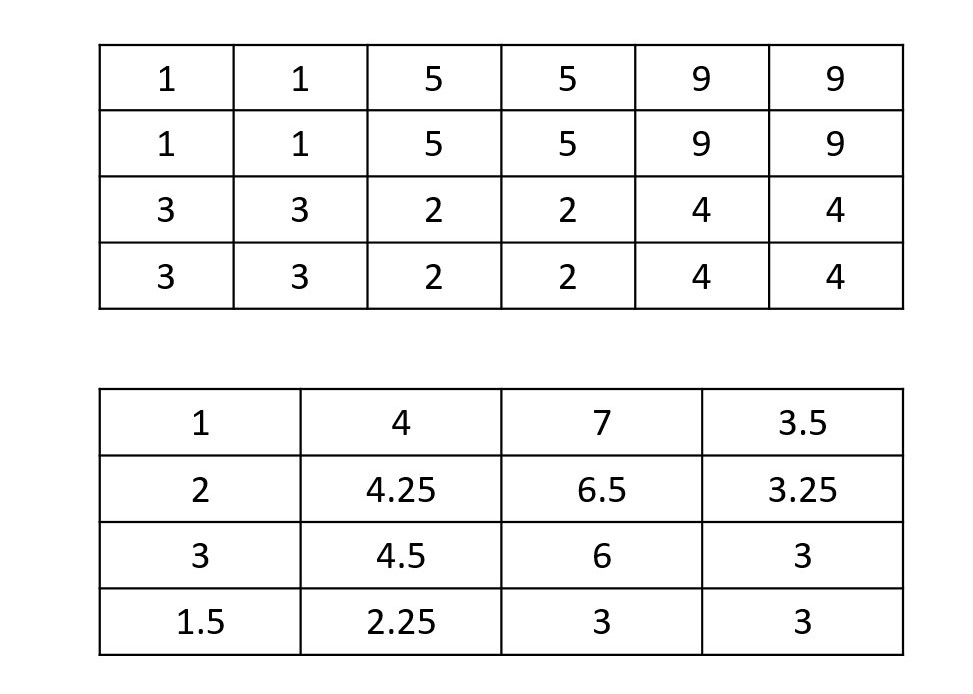
\includegraphics[width=200pt]{fig2.jpg}
	\label{fig_1}
	\end{center}

\section{}

We simply start by writing down the equations for the transition boundries and the reconstruction levels. These equations, can be easily derived by differentiating the MSE error.

$$t_{k} = \frac{r_{k-1} + r_k}{2}$$
$$r_k = \frac{\int_{t_k}^{t_{k + 1}} up(u)du}{\int_{t_k}^{t_{k + 1}}p(u)du}$$

In this particular case, we know that the probability distribution of the signal is Uniform. Therefore:
$$p(u) = constant = \frac{1}{32}$$

So we have:
$$r_k =  \frac{\int_{t_k}^{t_{k + 1}} u\frac{1}{32}du}{\int_{t_k}^{t_{k + 1}}\frac{1}{32}du} = \frac{\frac{1}{2}\frac{1}{32}u^2\vert^{t_{k+1}}_{t_k}}{\frac{1}{32}u\vert^{t_{k+1}}_{t_k}} = \frac{t^{2}_{k + 1} - t^{2}_{k}}{2(t_{k + 1} - t_k)} = \frac{t_{k + 1} + t_k}{2}$$

Additionaly, we have:
$$t_{k} = \frac{r_{k-1} + r_k}{2} = \frac{ \frac{t_{k + 1} + t_k}{2} +  \frac{t_{k-1} + t_k}{2}}{2}= \frac{t_{k} +   \frac{t_{k-1} + t_{k+1}}{2}}{2}\Rightarrow 2t_{k} = t_{k} +   \frac{t_{k-1} + t_{k+1}}{2}\Rightarrow t_k =  \frac{t_{k-1} + t_{k+1}}{2}$$

So:
$$t_{k+1} - t_k = t_k - t_{k - 1} $$
This means that the transition boundries are equaly distanced with each other with a distance that we call $q$ which is:.
$$q = \frac{t_{L + 1} - t_1}{L} $$

in the above mentioned equation $L$ is the number of levels, which in this case is equal to 4.
$$q = \frac{16 - (-16)}{4} = 8$$
So we have:
$$t_1 = -16$$
$$t_2 = -16 + 8 = -8$$
$$t_3 = -8 + 8 = 0$$
$$t_4 = 0 + 8 = 8$$
$$t_5 =  8 + 8 = 16$$

As for the reconstruction levels, we have:
$$r_1 = \frac{t_1 + t_2}{2} = -12$$
$$t_2 =  \frac{t_2 + t_3}{2} = -4$$
$$t_3 = \frac{t_3 + t_4}{2} = 4$$
$$t_4 = \frac{t_4 + t_5}{2} = 12$$

Because I have derived the values based on the equations in page 65 of the course slides, verification of the formulaes are not anymore necessary.

For the MSE we have:
$$E = \frac{q^2}{12} = \frac{64}{12} $$

Also:

$$ entropy: H = - \sum^{\L}_{k = 1} p(k)log_2 p(k) =- L \times \frac{1}{L}log_2 \frac{1}{L} = log_2 L = 2$$

\section{}

A unifrom quantizer with 32 levels, the number of bits required is equal to: $ B = log_2 32 = 5$
The SNR is equal to: 
$$SNR = \frac{E}{\sigma_{u}^2} = 10 log_{10} 2^{2 \times 5} = 30.103 dB$$
For the 64 Level case, we have: $ B = log_2 64 = 6$, and the SNR is:
$$SNR = \frac{E}{\sigma_{u}^2} = 10 log_{10} 2^{2 \times 6} = 36.123 dB$$

so the SNR will increase by \textbf{6.02 dBs}.

The bandwidth will increase. because  with more levels, we can detect the changes of the signal more precisely. That means that we can detect smaller changes in the signal which means that we can detect higher frequencies. So the bandwidth will likely increase. for example in the most basic case assume that we only have one level. In this case, every value of the signal, will map to one single value, and in the frequency domain, we only will have one dirac function ( $\delta(x)$). now if we increase the number of levels, the quantized signal will have more than one value (most likely, if the signal is not a constant signal) and this will in turn, increase the bandwidth of the function.

\section{}
\subsection{}
We use the fact that the transform coefficients ($v_{k,l}$) are equal to:
$$v_{k,l} = <F,H_{k,l}>$$

in which $<., .>$ is the frobinius inner product of two matrices:
$$<A, B> = Trace(A^TB) = \sum_{i}\sum_{j} a_{ij}b_{ij}$$

So:
$$v_{0,0}  =<F,H_{0,0}> = 4 \times \frac{1}{2} + 7\times \frac{1}{2}+ 3\times \frac{1}{2} + 5\times \frac{1}{2} = 9.5$$
$$v_{0,1}  =<F,H_{0,1}> = 4 \times \frac{1}{2} + 7\times \frac{1}{2} -3\times \frac{1}{2}  -5\times \frac{1}{2} = 1.5$$
$$v_{1,0}  =<F,H_{1,0}> = 4 \times \frac{1}{2} - 7\times \frac{1}{2}+ 3\times \frac{1}{2} - 5\times \frac{1}{2} = -2.5$$
$$v_{1,1}  =<F,H_{1,1}> = 4 \times \frac{1}{2} - 7\times \frac{1}{2}- 3\times \frac{1}{2} + 5\times \frac{1}{2} = -0.5$$
\subsection{}

$$\tilde{F} = 9.5 \times H_{0,0} -2.5 H_{1, 0} = \begin{bmatrix} 3.5 & 6 \\ 3.5 & 6\end{bmatrix}$$

\section{Practical Questions}

The answer to the practical questions, are included in the Jupyter notebook files, attached with this document.


















\end{document}